%(BEGIN_QUESTION)
% Copyright 2007, Tony R. Kuphaldt, released under the Creative Commons Attribution License (v 1.0)
% This means you may do almost anything with this work of mine, so long as you give me proper credit

Når du inspiserer PV- og SP-trender på en prosesskriver, legger du merke til dårlig reguleringskvalitet:

$$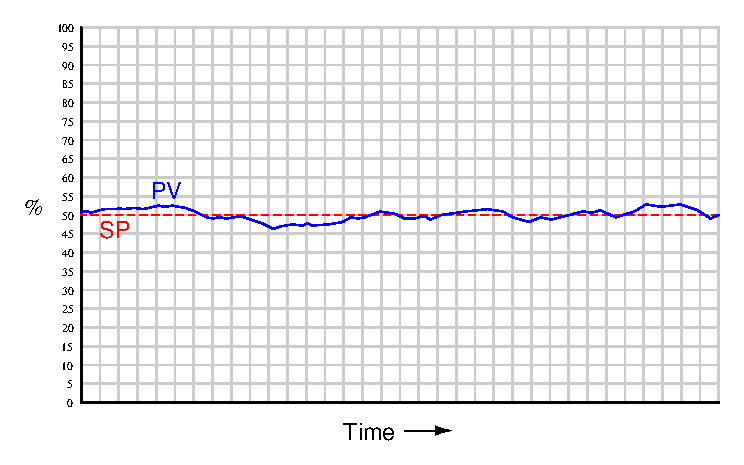
\includegraphics[width=15.5cm]{i01646x01.eps}$$

``Vandringen'' til prosessvariabelen (PV) rundt setpunkt kan skyldes for kraftig regulering fra regulatoren, eller skyldes lastvariasjoner i selve prosessen. Med andre ord kan ustabiliteten enten skyldes at regulatoren reagerer for aggressivt, eller at regulatoren ikke arbeider aggressivt nok til å motvirke endringer i prosesslasten.

Identifiser en enkel metode for å avgjøre hvilket scenario som er riktig. Hint: kontrollen er i de fleste tilfeller så enkel som å trykke på én knapp.

\underbar{file i01646}
%(END_QUESTION)





%(BEGIN_ANSWER)

Sett regulatoren i manuell modus og observer PV-trenden!

%(END_ANSWER)





%(BEGIN_NOTES)

Hvis PV vandrer enda mer når regulatoren står i manuell modus, vet du at regulatoren gjorde jobben sin, men kanskje ikke aggressivt nok. Hvis PV vandrer mindre eller slutter å vandre etter at regulatoren er satt i manuell modus, vet du at regulatorvirkningen faktisk gjør situasjonen {\it verre}.

Ikke alle tilfeller av overinnstilt regulator gir en pen sinusoscillasjon slik noen lærebøker viser! En overinnstilt regulator kan gi merkelige trendmønstre, særlig hvis prosessen har asymmetriske tidskonstanter (for eksempel en ovn som varmes opp raskere enn den kjøles ned).

Det {\it er} også mulig at PV oscillerer sinusformet uten at det er regulatorens feil. Hvis for eksempel en annen reguleringssløyfe i systemet er overinnstilt og oscillerer, kan den belaste prosessen du observerer med en sinusformet forstyrrelse, slik at mange prosessvariabler i systemet ``kruser'' tilsvarende.

%INDEX% Control, PID tuning: manual mode as a diagnostic tool

%(END_NOTES)
